\documentclass[10pt, a4paper]{aqademic}

\usepackage[english]{babel}
	\selectlanguage{english}

% Document packages

\usepackage[type=CC, modifier=by-nc-sa, version=4.0]{doclicense}
\usepackage{graphicx}
	\graphicspath{{img}}
\usepackage{hyperref}
\usepackage{url}

% Custom commands

\def\mysim{\raise.17ex\hbox{$\scriptstyle\mathtt{\sim}$}}

% Document settings

\author{Atanasio José Rubio Gil}
\title{Neosluger}

% Document composition

\begin{document}

\AqMaketitle[%
	author   = Atanasio José Rubio Gil,
	cover    = logo-ugr.png,
	org      = Office for Free Software,
	subtitle = User manual,
	url      = https://github.com/OSL-UGR/neosluger
]
\tableofcontents

\chapter{The service}\label{the-service}

\section{What is Neosluger?}\label{what-is-neosluger}

Neosluger\footnote{
	\url{https://github.com/OSL-UGR/neosluger}
} is a complete rewrite of the University of Granada's URL shortener Sluger\footnote{
	\url{https://github.com/OSL-UGR/sluger}
},
which stands for \textbf{S}hort \textbf{L}ink \textbf{UGR} (and \textit{e} is added as a pronunciation aid).
It is Free Software, which means that you are free to modify and distribute it as long as you do so bounded by the limits and obligations of its licence.

The old version offered a URL shortener, an API and public access stats for each short link.
This version renews the API and offers a QR code generator that can be freely used for any link, not only the officially shortened ones.
As with the old version, the URL shortener is only available for users accessing the service from the University of Granada's network, but all other services are available to the general public.
This is done to ensure that all links are created for purposes related to the University.

The new service is available in the same address as the original one: \url{https://sl.ugr.es/}

\section{The web interface}\label{the-web-interface}

\begin{figure}[ht!]
	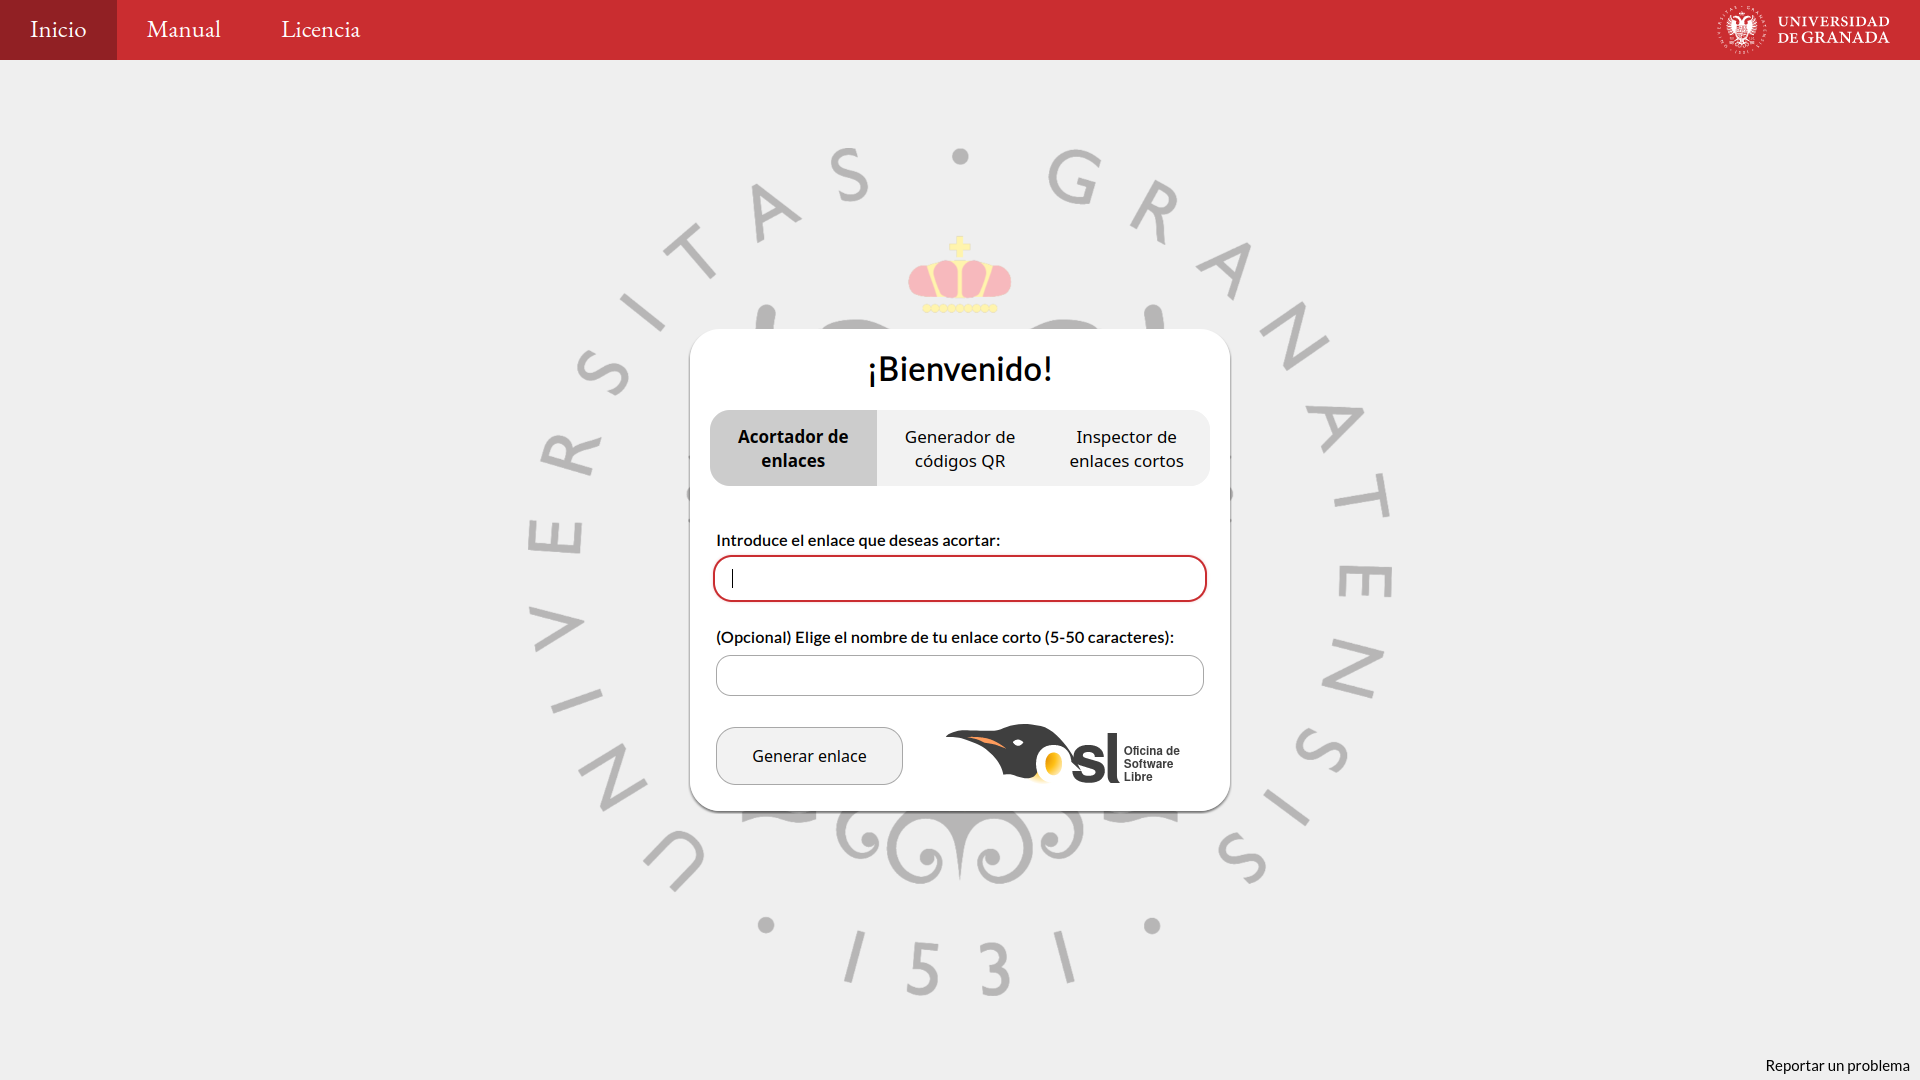
\includegraphics{web-index}
	\caption{Neosluger's index page.}
\end{figure}

Neosluger's web interface consists of three tabs:
The index tab (\textit{Inicio}) is the one the user sees first and contains the URL shortener (\textit{Acortador de enlaces}), the QR code generator (\textit{Generador de códigos QR}) and the shortened URLs inspector (\textit{Inspector de enlaces cortos}).

The manual page contains instructions for the URL shortener (\textit{Acortador de enlaces}), the QR code generator (\textit{Generador de códigos QR}) and the API.
The licence page contains the service's licence, a link to the original text by GNU, a raw version of the licence and a link to Neosluger's repository.
Every pages contains a report button (\textit{Reportar un problema}) that guides the user to a report page where they can get in contact with the University's Office for Free Software to change or delete a link or to have a feature fixed as soon as possible.

\begin{figure}[ht!]
	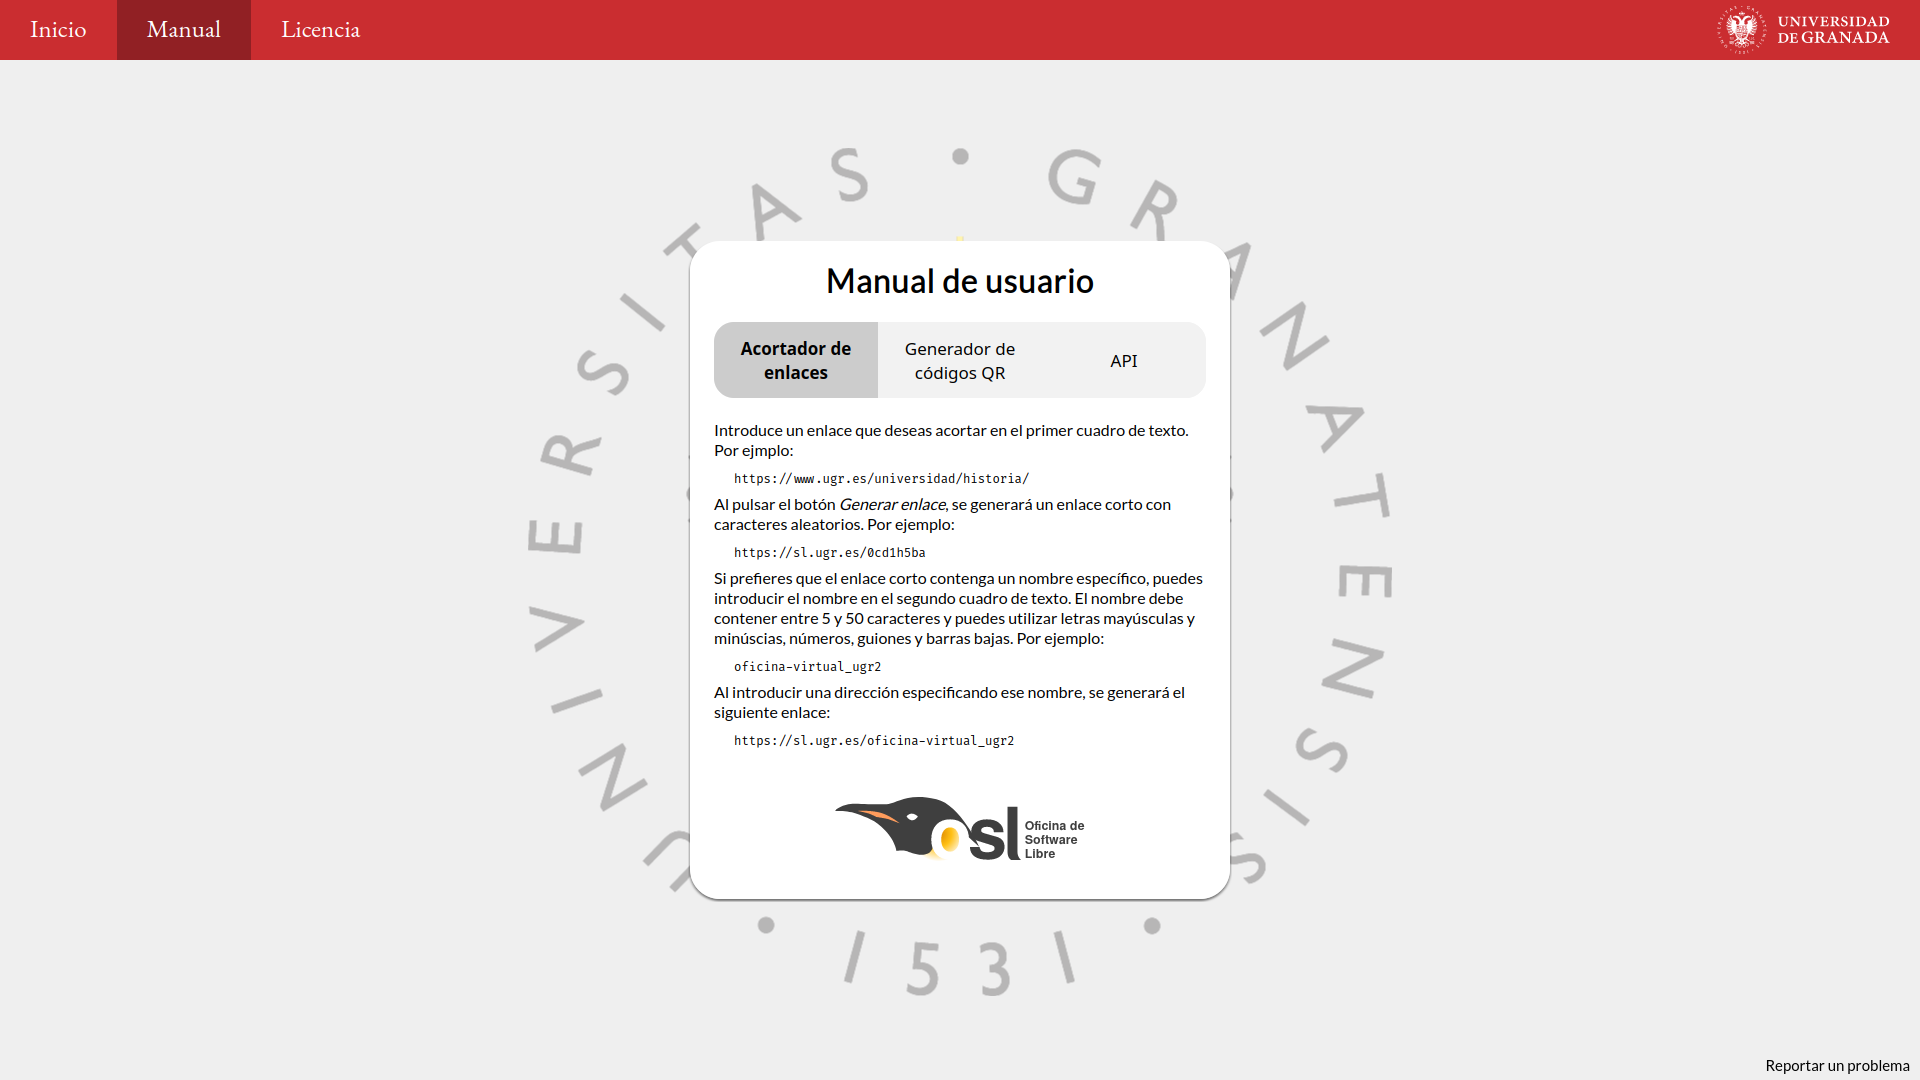
\includegraphics{web-man}
	\caption{Neosluger's manual page.}
\end{figure}

\begin{figure}[ht!]
	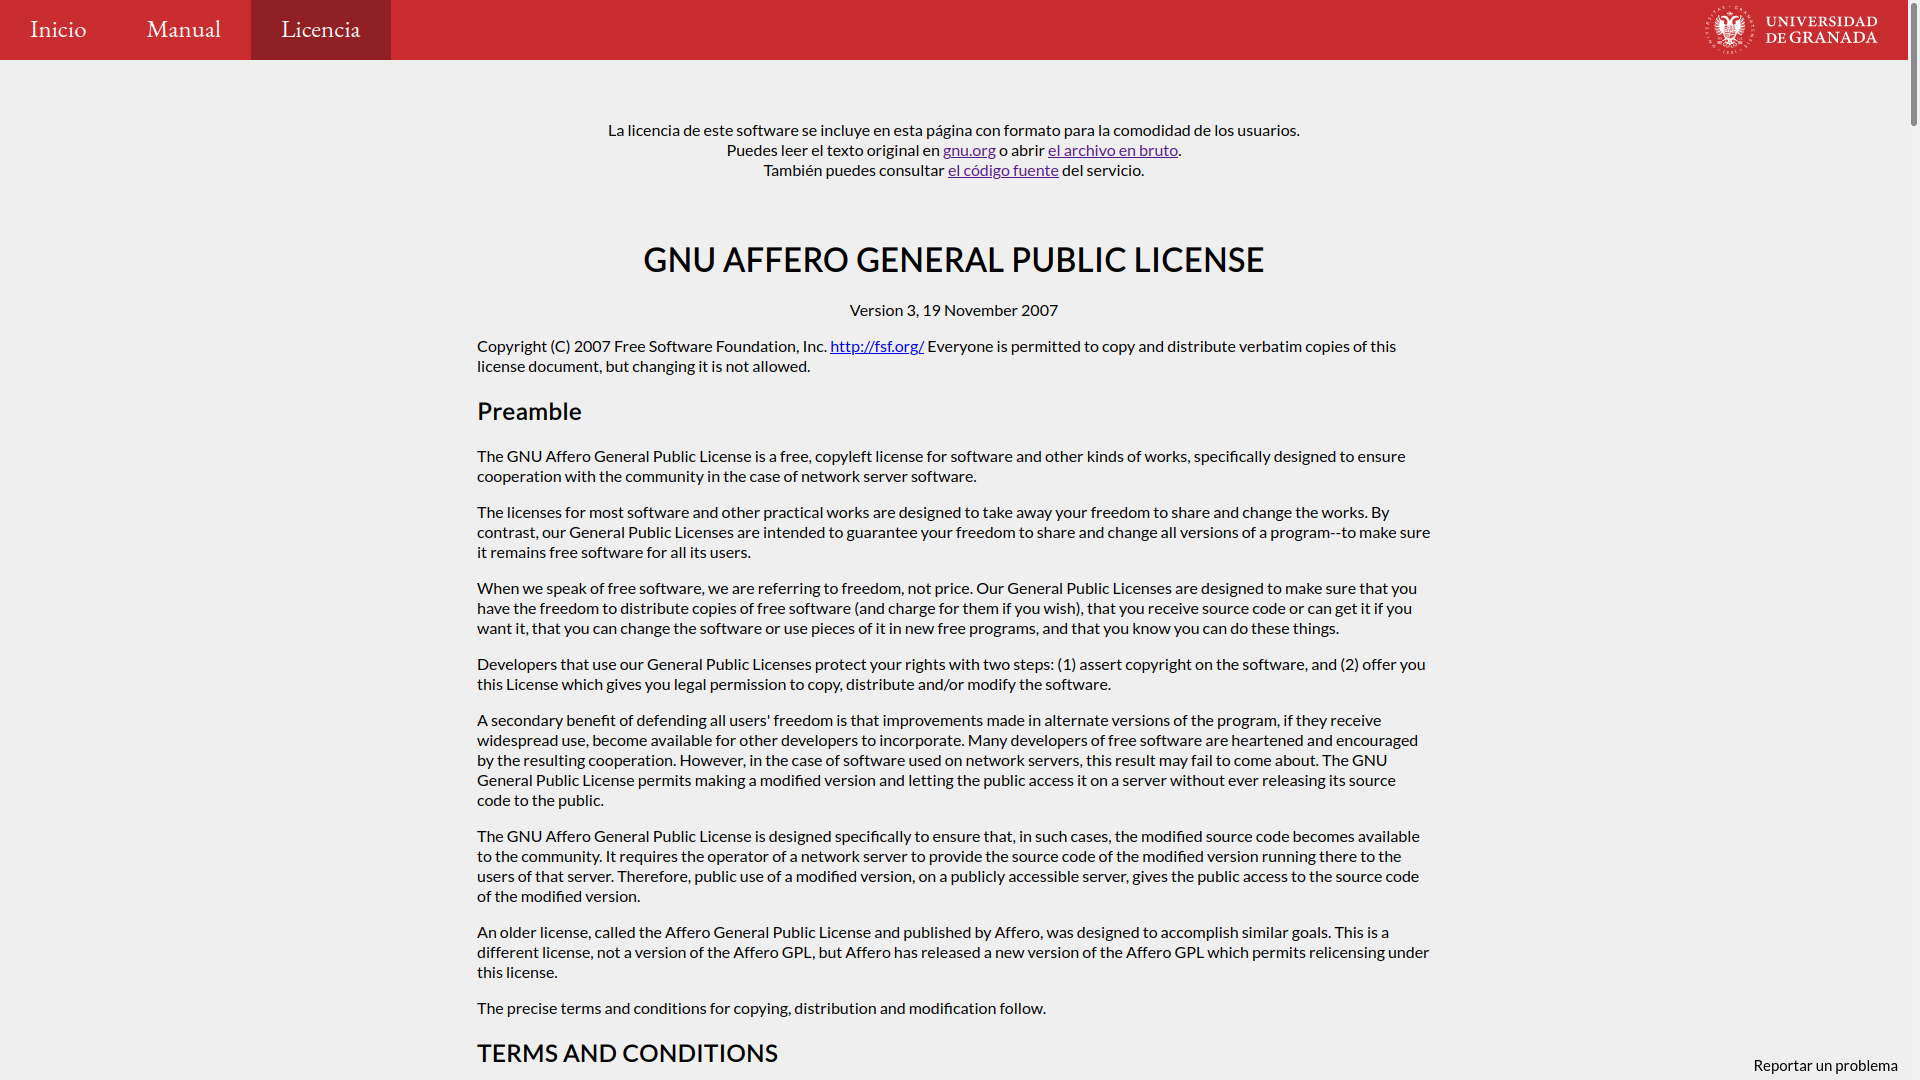
\includegraphics{web-licence}
	\caption{Neosluger's licence page.}
\end{figure}


\section{The API}\label{the-api}

Another way of accessing the service is through its API (Application Programming Interface), that allows other programs to request a short link from the service without having to use the web interface.
Its use will be further described in its own section.
\begin{figure}[ht!]
	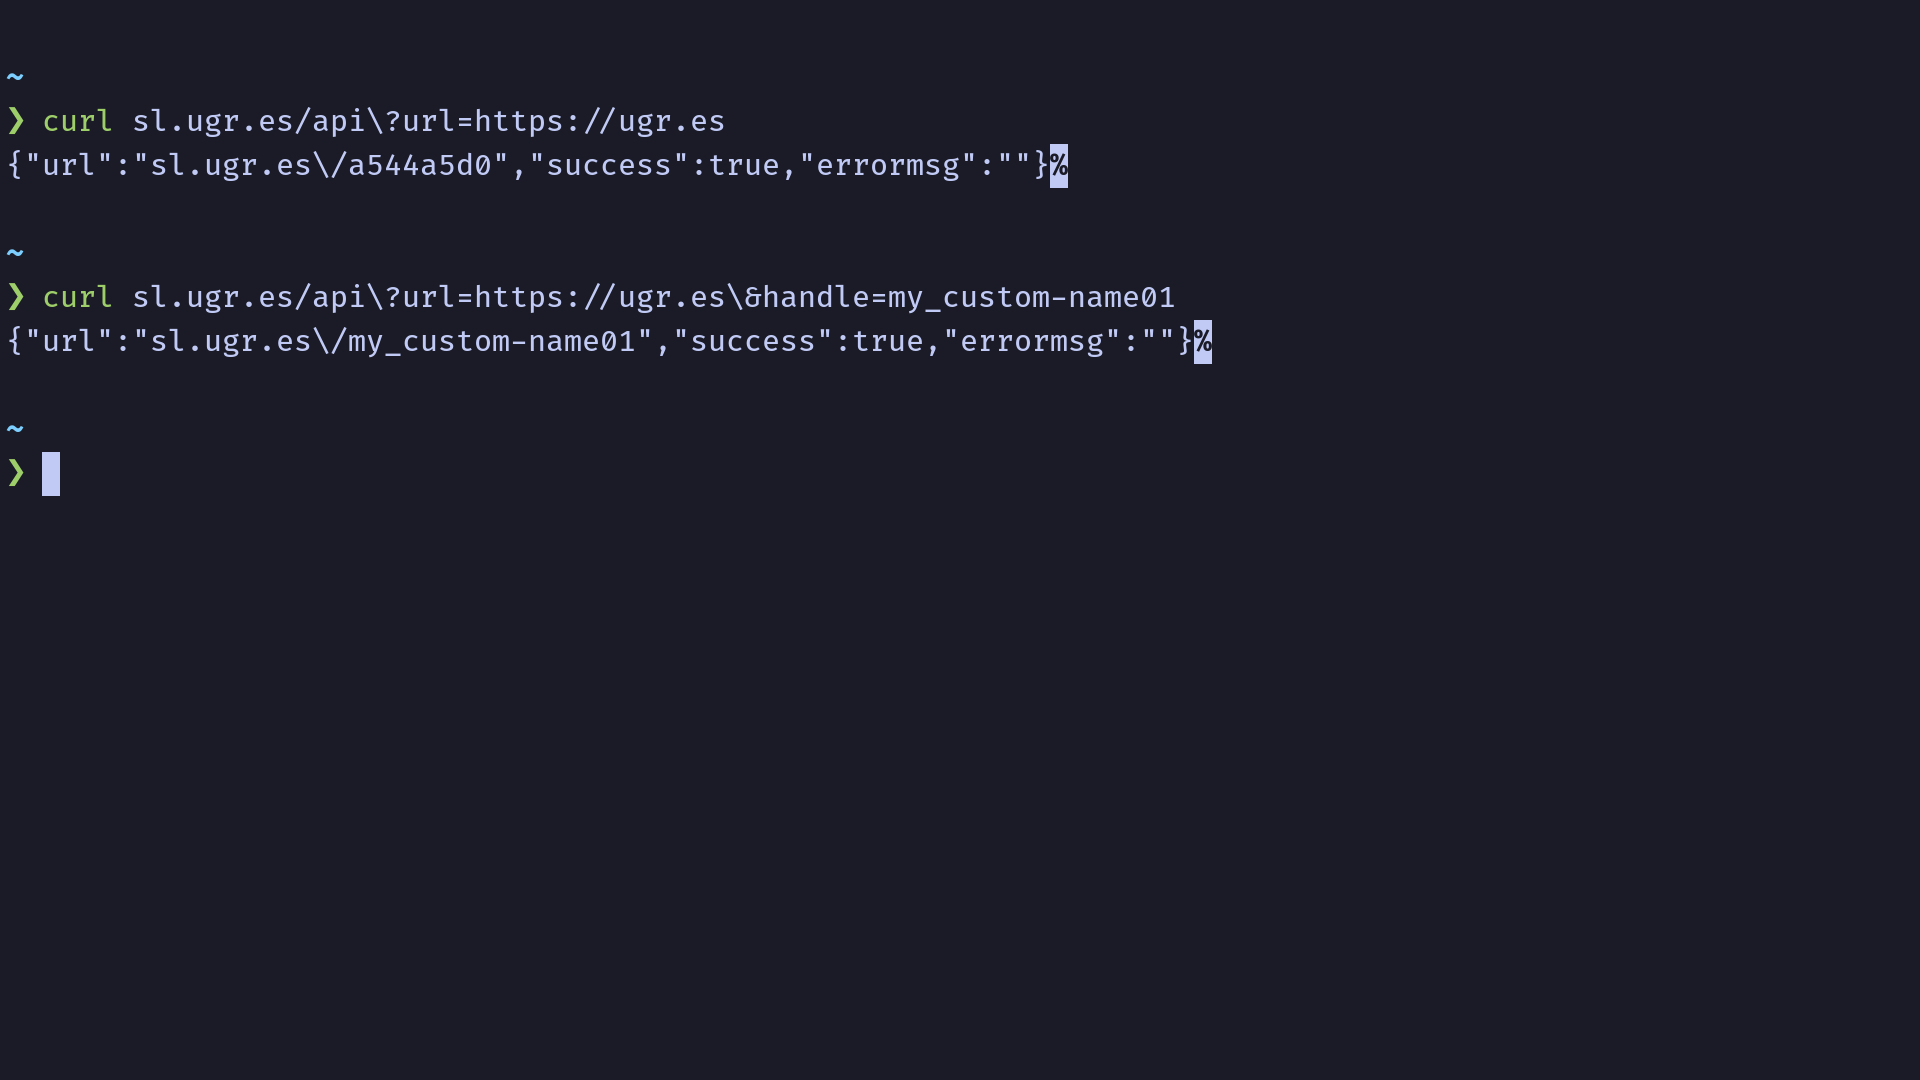
\includegraphics{api-curl}
	\caption{Short URLs creation through the API.}
\end{figure}

\chapter{Setting up the server}\label{setting-up-the-server}

\section{Configuration files}\label{configuration-files}

Neosluger is configured to run in an Nginx server.
It can be configured to run with Apache, but this is not officially supported.
The server configuration file is available in Neosluger's repository \texttt{conf/} directory and is named \texttt{neosluger.conf}.
To install it, add it to \texttt{/etc/nginx/sites-enabled/neosluger.conf} and modify it to match you system's settings as required.
The default directory to host Neosluger is \texttt{/var/www/neosluger/src}.
If you decide to place it in any other directory, you must change the \texttt{root} directory to match the new path.
Finally, add the following directive in \texttt{/etc/nginx/nginx.conf}:

\begin{lstlisting}[language=sh]
http {
	# Add this include directive in the body of the already existing http block:
	include /etc/nginx/sites-enabled/neosluger.conf;
}
\end{lstlisting}

% TODO: Ubuntu shenanigans

\section{Dependencies}\label{dependencies}

Neosluger requires \texttt{php}, \texttt{php-gd}, \texttt{php-fpm} \texttt{mongodb} and \texttt{php-mongodb} to run.
You can easily install it with your distro's package manager, but bear in mind that the packages may have different names depending on the repository you are accessing.
After installing PHP, install \texttt{composer} to manage Neosluger's internal dependencies.
The latest version at the time of writing is \texttt{v2.2.6} and it is the version that has been used to develop Neosluger.
If the version provided by your package manager is lower than \texttt{v2.0} or throws warnings when installing the internal dependencies, reinstall \texttt{composer} manually following the official instructions\footnote{
	\url{https://getcomposer.org/download/}
}.

To install Neosluger's internal dependencies, move to the \texttt{src/} directory and install them with \texttt{composer}:

\begin{lstlisting}[language=sh]
cd src/
composer install
\end{lstlisting}

This will install the latest versions of the dependencies.
To install them with the latests tested versions, copy the \texttt{composer.lock} file inside \texttt{src/}, next to where \texttt{composer.json} is.
This file contains metadata about the latest update so that running \texttt{composer install} will download the correct dependencies' versions to match the locked system.
In short, if it works in my machine, I can send you my lock file to make it work in yours too.

\section{Setting up the database}\label{setting-up-the-database}

Neosluger stores all its data in a local MongoDB database.
Its address is defined in \texttt{php/const.php} and points to the local database set up by the MongoDB service.
You can change it if your instance uses a database in a different location.
When the database is up, run \texttt{conf/migrate.php} to set up the database indices.

\subsection{Benchmarking}\label{benchmarking}

You can run \texttt{conf/benchmark.sh} to test the time spent in subsequent API calls.
Run \texttt{conf/benchmark.sh --help} for more details.

\section{Starting the service}\label{starting-the-service}

With the server correctly configured and all dependencies installed, you can now start the \texttt{systemd} services required to run Neosluger:

\begin{lstlisting}[language=sh]
sudo systemctl start nginx php-fpm mongodb
\end{lstlisting}

You can also use the following command to automatically report errors:

\begin{lstlisting}[language=sh]
sudo systemctl restart nginx php-fpm mongodb || sudo systemctl status nginx
\end{lstlisting}

After this, you should be able to access the server with the IP address configured by Nginx.

\section{Cache directory}\label{cache-directory}

QR codes are saved in a cache directory to be presented to the user and be downloaded by them.
Its route is set in \texttt{pages/url-result.php} and defaults to \texttt{src/cache/qr/}.
You may be forbidden from writing into this directory if Neosluger is hosted in \texttt{/usr/}.
If that is the case, please refer to this ServerFault answer: \url{https://serverfault.com/a/997496}.

To use the directory, you need to give the user running PHP permission to write into it.
Neosluger will create the cache directory if it does not exist, so you should give write permissions to \texttt{src/}.
This may look like the following:

\begin{lstlisting}[language=sh]
chown -R "$USER":http src/
chmod -R g+w src/
\end{lstlisting}

\section{Testing the service}\label{testing-the-service}

Once Neosluger is running in your server, you can run its test suites using PHPUnit to ensure that the system won't throw any errors at runtime:

\begin{lstlisting}[language=sh]
cd src/
vendor/bin/phpunit tests
\end{lstlisting}

The test suites also acts as a complete reference for any developer who wishes to extend the system.

\subsection{Directory permissions clash}

The web server is ran by the user \texttt{http}, while the tests are ran by \texttt{"\$USER"}.
This means that whoever gets to create the cache directory first gets all the permissions to read and write to it.
To solve this, you \textbf{must} edit the cache directory's owners in two cases:

\begin{itemize}
\item
	After creating the cache directory from running the test suites so that the web server can create the codes.
\item
	After creating the cache directory from a web server response so that the tests can pass.
\end{itemize}

To update the owners you just need to \texttt{chown} the deepest directory:

\begin{lstlisting}[language=sh]
cd src/
chown "$USER":http cache/qr
\end{lstlisting}

The directory's permissions are set to \texttt{775} by the service.

\chapter{Resolving links}\label{resolving-links}

\section{Server configuration}\label{server-configuration}

The server configuration file installed in \S\ref{configuration-files} defines the first steps the server has to take to respond to the users' petitions.
Every time a user tries to access the service, they do it with an HTTPS petition to \url{https://sl.ugr.es/}.
When the server receives a petition, it opens the \texttt{location /} block in the configuration file and looks inside it to find a page they can serve the user to respond to their petition:

\begin{lstlisting}
location / {
	try_files $uri /php/resolver.php?$args;
	index pages/index.php;
}
\end{lstlisting}

The \texttt{try\_files} directive tries to find a find a page corresponding to the requested URI.
For example, if the user asks for \texttt{https://sl.ugr.es/licence}, it will try to find a page that can be served for the URI \texttt{licence}.
It is guaranteed that \texttt{\$uri} will fail, since all pages are inside the \texttt{pages/} directory, which means that every time the user asks for a page they will be redirected to \texttt{/php/resolver.php}.
The \texttt{?\$args} suffix means that any arguments passed along with the URI will be passed to the resolver so that they can be used by the pages it redirects them to.
We will discuss the resolver with greater depth in \S\ref{the-resolver-script}.
The \texttt{index} directive lets the server know what to load when the user accesses the service directly, i.e. \url{sl.ugr.es}.

The \texttt{location \mysim\char`\\.php\$} block does the same as the previous block, but tries \texttt{\$fastcgi\_script\_name} instead.
This directive is used instead of \texttt{\$uri} because \texttt{fastcgi} is the protocol that effectively loads the PHP service.

Finally, the \texttt{error\_page} directive redirects all \texttt{404} errors to \texttt{/pages/404.php}.
In theory, this directive is not required because the resolver sends lost users to the 404 page, but nobody is going to complain about a little resilience and loading the custom 404 page is much more elegant than serving the default one.

\begin{lstlisting}
error_page 404 /pages/404.php;
\end{lstlisting}

\section{The resolver script}\label{the-resolver-script}

Every petition is forwarded to this script, which parses the URI and finds the best page to serve the user or redirects them from a short link.
The script was written for scalability reasons given the requisites of Neosluger:

\begin{itemize}
\item
	The user must be able to access pages inside the site without having to know the absolute path.
	E.g. \texttt{sl.ugr.es/man} must be able to serve \texttt{pages/manual.php}.
\item
	The user must be able to use a short URL to be automatically redirected and prepend \texttt{stats/} to the URL handle to inspect it and see its usage statistics.
\item
	The users must not be able to access the different pages from their location in the server directory tree.
	This improves the service's security.
\item
	The old API must still work, even though it will always throw an error.
\end{itemize}

If the URIs were resolved by the server configuration file, every time a new page was added to the service it would need to be modified and it would get clobbered really fast.
Instead, we let the resolver script handle this for us and check whether the user is accessing a page within the service or wants to be redirected from a short URL.

The resolver follows these steps to serve the user the page they expect:

\begin{lstlisting}
Parse URI received from the server

if a maching page is found in pages/*.php:
	render the page
otherwise, if the URI is NOT a handle found in the database:
	if it refers to the old API:
		serve an API deprecation error message
	otherwise
		serve the 404 page
otherwise, if the handle was found in the database:
	Prevent the user from caching this page to register all accesses to the link
	Register the access
	Redirect the user to their destination
\end{lstlisting}

The order of the paths is unusual because checking if a URL wasn't found in the database is done by a call to \texttt{\$url->is\_null()} and \texttt{if} statements are written so that their conditions never contain a negation, which is easier to reason about.

\section{Rendering pages}\label{rendering-pages}

All pages in \texttt{pages/*.php} \textbf{must} contain a \texttt{render} function to act as the main function of the page and call them at the end of the file.
This way, when the resolver includes them, the \texttt{render} function is called automatically by the page.

Pages are rendered using Twig, a templating engine that lets Neosluger reuse interface code and be much easier to maintain.
Twig directives are specified inside \texttt{\{\% \%\}} and \texttt{\{\{ \}\}} blocks.
The first type of blocks are used for reserved words like \texttt{[end]block}, \texttt{[end]if} and to call objects' member functions like \texttt{url.is\_null()} (notice the \texttt{.} operator instead of \texttt{->}).
The second type of blocks expands the value inside the braces.
For example, if we have a variable \texttt{\$name = "Taxo"}, \texttt{<p>My name is \{\{ name \}\}.</p>} will be expanded to \texttt{<p>My name is Taxo.</p>}

To render a page, \texttt{Twig->render()} must be called from an \texttt{echo} statement.
It receives the route of the HTML file it has to render and an associative array of objects where the names are the variables used by the template.


\end{document}
